\documentclass[12pt] {report} %[conference]{IEEEtran}
\renewcommand{\baselinestretch}{1.2} 

%Packages
\usepackage{graphicx}
\usepackage{amsmath}
\usepackage{amssymb}
\usepackage{upgreek}
\usepackage{cite}
\usepackage{refstyle}
\usepackage{caption}
\usepackage{subcaption}
\usepackage{float}
\usepackage{fullpage}
\usepackage{tikz}
\usepackage{tkz-berge}
\usepackage{listings}

\graphicspath{{Images/}}

\definecolor{mygray}{rgb}{0.95,0.95,0.95}

\begin{document}
\tableofcontents
%\listoffigures

\lstset{
	language=c++,
	backgroundcolor=\color{mygray},
	%commentstyle=\color{mygreen}
	frame=single,
	keywordstyle=\color{blue},
	numbers=left,
	rulecolor=\color{black},
	title=\lstname 
	}
	
	\begin{titlepage}
	    \begin{center}
	        \vspace*{1cm}
	        
	        \Huge
	        \textbf{Monte Carlo Simulations in the 2-dimensional Ising Model.}
	        
	        \vspace{2cm}
	        
	        \textbf{Anthony Bourached}\\
	        Supervisor: Professor Stefan Sint
	        
	        \vfill
	        
	        A thesis presented for\\
	        module MA4492
	        
	        \vspace{0.8cm}
	        
	        \includegraphics[width=0.4\textwidth]{trinity}
	        
			\large 
	        School of Mathematics\\
	        Trinity College Dublin\\
	        Ireland\\
	        15 Feburary 2015
	        
	    \end{center}
	\end{titlepage}

	\begin{abstract}
		We perform Monte Carlo simulations on the 2-dimensional Ising model in a zero magnetic field, using the Metropolis and Wolff Cluster algorithms to obtain computational results for thermodynamic quantities and the dynamic critical exponents of the algorithms. The Ising model in 2-dimensions and zero magnetic field undergoes a second order phase transition from a phase with no magnetisation to one with spontaneous magnetisation. This phase transition is modelled by our simulations with the behaviour of magnetisation, energy, magnetic susceptibility and heat capacity at phase transition all being accurately valued. We used finite size scaling of the lattice at critical temperature to derive the value of the dynamic critical exponent for both algorithms of $z = 2.11 \pm 0.073$ for Metropolis and $0.47 \pm 0.051$ for Wolff Cluster which compares well with accepted quantities of $z_{metropolis} = 2.17$ and $z_{cluster} = 0.52$. Critical exponents of derived observables magnetic susceptibility ($\gamma$) and heat capacity ($\alpha$) were found to be $\gamma = 1.76 \pm 0.023$ and $\alpha = 0.29 \pm 1.5$. $\gamma$ compared well with the accepted value of $\gamma = 7/4$. The discrepancy of $\alpha$ from the accepted value 0 was discussed.
	\end{abstract}
	
	\chapter{Introduction}
	 
	
		\paragraph{}
			The Ising model, named after Ernst Ising who first studied it in 1923, has played a central role in the development of statistical physics and quantum field theory \cite{anagnostopoulos} and is one of the most famous statistical systems. Of particular interest is the two dimensional Ising model which is complicated enough to possess non-trivial properties yet still simple enough to have an exact analytical solution. For several years the Ising model was considered as a greatly over-simplified representation of intermolecular forces and as being inapplicable to any real systems \cite{history}. In fact Ernst Ising gave up on his research in physics after he believed that he had proved that the model had no physicsal usefulness, yet twenty years later he was to become famous as a result of his work on the model \cite{history}.
		\paragraph{}
			In 1923 Ising showed that the one-dimensional model does  not exhibit magnetic behaviour in the absence of a magnetic field \cite{blair}. He assumed that this result could be extrapolated in higher dimensions. However, this was incorrect. The Ising model zero magnetic field, in two or more dimensions, undergoes a second-order phase transition at a critical temperature $T_c$ from a disordered, high temperature state with zeroed magnetization; to an ordered, low temperature state that has spontaneous magnetization. This is the case only for a finite size lattice; in the thermodynamic limit there is no spontaneous magnetization.
		\paragraph{}
			It was only in the late 1940s that the Ising model began to rise in popularity. The explicit solution of the two-dimensional problem involved such difficult mathematics that it stumped all physicists who attempted it. In fact, it was a chemist (Onsager 1948) who found the full analytical solution to the two dimensional model in zero magnetic field,  which remains one of the most important achievements in statistical mechanics. The result is interesting from a physical point of view since it is the simplest, most phenomenologically interesting, model of a ferromagnetic material. Due to universality, the model describes also the liquid/vapor phase transition at the triple point \cite{anagnostopoulos}. 
		\paragraph{}
			Another approach to studying the Ising model, which is the focus of this report, is Monte Carlo simulations. These are highly efficient computational methods for solving dynamic systems in thermal equilibrium. The goal of this report is to examine in detail the errors and efficiencies of two Monte Carlo methods which greatly differ in their approach to solving the model. Their strengths and weaknesses will be compared and contrasted. The two algorithms are the local change Metropolis algorithm and the non-local Wolff Cluster algorithm.
		\paragraph{}
			In Chapter \ref{chapter:statistical physics} we shall review the fundamentals of statistical physics that are essential in understanding the Ising model and, in section \ref{sec:Ising model}, how this basis in statistical physics leads us to derive bulk properties of the Ising model from the hamiltonian of the system.
		\paragraph{}
			 Chapter \ref{chapter:monte carlo simulations} shall give an introduction to the Monte Carlo computation methods and a detailed discription of the algorithms used. We will also discuss in detail the method of deriving bulk properties from our functioning algorithms and how to become confident that our results are representative of the equilibrium state of the system. We shall further discuss the concept of autocorrelation and how this effects our results. Chapter \ref{chapter:monte carlo simulations} will be concluded with a discussion of how error analysis was conducted in this project.
		\paragraph{}
			In Chapter \ref{chapter:testing_algorithms} we shall discuss an exact (non-statistical) computational solution to the model which, for reasons that shall be discussed is only practical for very small systems. We shall also compare these exact results to those found by our statistical approach to ensure that they are in strong agreement within our calculated margin of error.
		\paragraph{}
			In Chapter \ref{chapter:simulations} we shall present a discussion on data produced by our simulations. We shall use the methods described in \ref{chapter:monte carlo simulations} to calculate expectation values of various observables and their associated errors. In particular we shall focus on the computation of autocorrelation times of the algorithms and how they handle critical slowing down. This is expected to be the greatest variant between the algorithms as the Wolff Cluster algorithm was introduced as an effective way of beating the effects of critical slowing down. We shall further discuss the implications of these comments on the efficiencies of the system and our choice of algorithm later.
		\paragraph{}
			Finally, in Chapter \ref{chapter:conclusions} the overall achievements and observations of this project will be summarised. The most important discovery will be highlighted and its implications underlined. This will conclude the project.
			
	
	\chapter{Statistical Physics} \label{chapter:statistical physics}
	
		\section{The Need for Statistical Physics}  \label{sec:basic_statistical_physics}
		
			\paragraph{}
				A simple macroscopic system generally has between $10^{23}$ and $10^{44}$ number of degrees of freedom. This could describe anything from water vapour to an entire planet. Hence, it is impractical to determine exact results from the evolution of the system. It is enough, however, to know a small number of bulk properties of the system in order to have a useful description of it.
			\paragraph{}	
				For example, we have sufficient information from the energy and density of a fluid without needing to know the position; momentum; energy and angular momentum of each individual molecule which would provide us with more information than we need, or than it would be possible to analyse. It is possible to use Monte Carlo simulations to find these bulk properties from the hamiltonian of the system.
			\paragraph{}
				We can consider a system to have $N$ discrete states each with a discrete energy $E_0 < E_1 < ... < E_\mu < ... < E_{N-1}$. This system is in contact with a termal resevoir of temperature T. When the system is in thermodynamic equilibrium with the resevoir, its bulk properties are described by the canonical ensemble. Weights describe the probability for the system to be in state $\mu$ at time $t$. The probability for state $\mu$ with energy $E_{\mu}$ is given by $p_\mu$ and is the connection between the microscopic and statistical descriptions of the system. The Boltzmann distribution gives: 
				
			\begin{align}
				p_{\mu} = \frac{e^{-\beta E_\mu}}{Z}  \label{eq:canonical_ensemble}
			\end{align}
			
				$\beta$ is the known as the coupling temperature and is given by:
			
			\begin{align}
				\beta = \frac{1}{kT}			\label{eq:beta}
			\end{align}
			
			\paragraph{}
				Where $k$ is Boltzman's constant. $\beta$ is refered to as the inverse temperature and is sometimes used as the independent variable in calculation rather than T. In this paper, it is indeed $\beta$ to which we often refer. Where high temperature refers to low $\beta$ and low temperature refers to high $\beta$. As a matter of convention we also choose natural units i.e. $k=1$.
		
			\paragraph{}
				Z is a normalising factor known as the partition function. It encrypts all the thermodynamic information about a system.
				
			\begin{align}
				Z = \sum_{\mu}^{}e^{-\beta E_{\mu}} 	\label{eq:partition_function}
			\end{align}
			
			\paragraph{}
				All thermodynamic properties of a system can be calculated from the partition function for that system. It is simply the sum of the weights of each state of the system. We can see that for a very high $\beta$ ($T \rightarrow 0$) equation (\ref{eq:canonical_ensemble}) becomes $p_\mu = 1/(\text{number of states})$ ie. each state equally likely. 
			
			\paragraph{}
				Thermodynamic systems have a stocastic (non-deterministic) character. Thus if we want to measure a physical quantity, or \textit{observable} (O), we compute the thermal average, as the probability of measuring a quantity to take a value significantly different from its average is ridiculously small. This average is referred to as the expectation value of the observable $\langle O \rangle$. The expectation value is found by averaging the observable over all possible states of the system, weighted by Boltzmann probabilities: 
				
			\begin{align}
				\langle O \rangle = \dfrac{1}{Z} \sum_{\mu} O_\mu e^{- \beta E_\mu}	\label{eq:expectation_value}
			\end{align}
			
			\paragraph{}
				where $O_\mu$ is the value of O in state $ \mu $.
				
			\paragraph{}
				The observables of particular interest in this paper are magnetization and the internal energy of the system to which we, for convenience, refer to simply as energy. For a statistical system we may calculate the expectation values of these observables using equation (\ref{eq:expectation_value}).
				
			\begin{align}
				\langle M \rangle =& \dfrac{1}{Z} \sum_{\mu} M_\mu e^{- \beta E_\mu}  \label{eq:expectation_value_mag}\\
				\langle E \rangle =& \dfrac{1}{Z} \sum_{\mu} E_\mu e^{- \beta E_\mu}	\label{eq:expectation_value_energy}
			\end{align} 
			
			\paragraph{}
				These quantities are almost always measured as other quantities can be dervied from them. Such as the susceptibility:
				
			\begin{align}
				\chi =& \: k \beta (\langle M^2 \rangle - \langle M \rangle^2)	\label{eq:susceptibility}
			\end{align}
				
				\paragraph{}
					and the heat capacity:
					
			\begin{align}
				C =& \: k \beta^2 (\langle E^2 \rangle - \langle E \rangle^2)		\label{eq:heat_capacity}
			\end{align}
			
			which are expressed above as the variation of magnetization and energy respectively and are hence refered to as derived observables since when we calculate them in this way it it not necessary to take and further measurements from the system. k is a constant specific to the system.
				
		
		\section{The Ising Model} \label{sec:Ising model}
		
			\paragraph{}
				Consider a d-dimentional lattice with a scalar valued elementary spin at each lattice point of $s_i = \pm 1$. This may be considered to be an atom or a magnet due to the universality of the model. Each side is of length L giving a total $N = L^d$ number of spin sites. Sites are connected to one another via links to their nearest neighbours with whom they directly interact. This spin-spin interaction is what determines the dynamics of the system.
				
			\paragraph{}
				At the boundary of the lattice periodic boundary conditions are usually employed such that the rightmost site's nearest neighbour to the right is the leftmost site. This is clearly illustrated in figure \ref{fig:ising_model}.
			
			\begin{figure} 
			\centering
			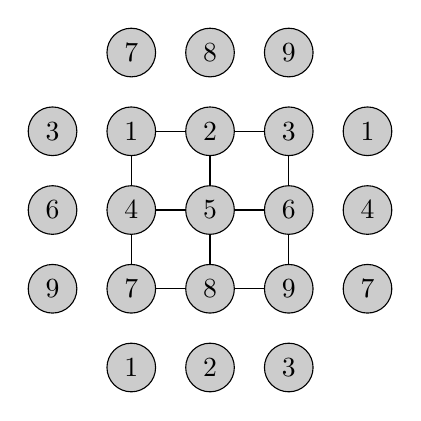
\begin{tikzpicture}[darkstyle/.style={circle, draw, fill=gray!40, minimum size=10}] 	
  				\foreach \x in {0,...,2}
			    \foreach \y in {0,...,2} 
			       {\pgfmathtruncatemacro{\label}{\x + 7 - 3*\y }
			       \node [darkstyle]  (\x\y) at (1*\x,1*\y) {\label};} 
			     
			    \foreach \x in {0,...,2}  
				    {\pgfmathtruncatemacro{\label}{\x + 7}
				 	\node [darkstyle]  () at (1*\x ,3) {\label};}
				 	
			    \foreach \x in {0,...,2}  
				    {\pgfmathtruncatemacro{\label}{\x + 1}
				 	\node [darkstyle]  () at (1*\x ,-1) {\label};}
			 	
   				\foreach \x in {0,...,2}  
				    {\pgfmathtruncatemacro{\label}{-\x*3 + 7}
				 	\node [darkstyle]  () at (3 ,1*\x) {\label};}	
				 	
   				\foreach \x in {0,...,2}  
				    {\pgfmathtruncatemacro{\label}{-\x*3 + 9}
				 	\node [darkstyle]  () at (-1 ,1*\x) {\label};}		 
			
			  \foreach \x in {0,...,2}
			    \foreach \y [count=\yi] in {0,...,1}  
			      \draw (\x\y)--(\x\yi) (\y\x)--(\yi\x) ;
			\end{tikzpicture} 
			\caption{2-dimentional L = 3 lattice, $N = L \times L = 9$. Links between nearest neighbours are seen as lines connecting sites and periodic boundaries are shown for this small lattice. Note, for illustration purposes the links across the boundary are not shown here but do exist.}
			\label{fig:ising_model}
			\end{figure}
			
			\paragraph{}
				The Hamiltonian for the Ising model is given by:
				
			\begin{align}
				H = -J \sum_{\langle i,j \rangle}s_i s_j - B \sum_{i}s_i		\label{eq:full_hamiltonian}
			\end{align}
			
			\paragraph{}
				where B is the external magnetic field. We consider the 2-dimensional ising model in a zeroth magnetic field (B=0) and so the Hamiltonian is given by:
				
			\begin{align}
				H = -J \sum_{\langle i,j \rangle}s_i s_j		\label{eq:hamiltonian}
			\end{align}
			
			\paragraph{}
				where the notation $\langle i,j \rangle$ is a sum over nearest neighbours for each given point, or in other words: $\sum_{\langle i,j \rangle}s_i s_j = \sum_{i, j}(s_{i,j} \cdot s_{i, j+1} + s_{i,j} \cdot s_{i+1, j})$. We only take the two links (up and right in this case) since once we have summed over all spins we will have accounted for each link; two vertices are connected by one link and four links intersect at one vertex:
				
			\begin{align}
				2N_l  = 4N \Rightarrow N_l = 2N 		\label{eq:number_of_links}
			\end{align}
				
			\paragraph{}
				J is the exchange energy (for interaction between spins). If $J > 0$ then the energy of the system is lowered when spins align which is known as ferromagnetic behaviour. $J < 0$ causes the system to have lowest energy when spins are anti-parallel, referred to as anti-ferromagnetism. The system is considered to be in thermodynamic equilibrium when its energy reaches a steady state minimum and for this reason the system tends to ferromagnetism for $J > 0$ and paramagnetism for $J < 0$ for a system with a non-zero external magnetic field.
				
				\paragraph{}
					We can consider the total Magnetisation of the system in state $\mu$ to be given by:
				
			\begin{align}
				M =	\left| \sum_{i}s_i \right|	\label{eq:magnetization}
			\end{align}
			
			\paragraph{}
				The probability of the appearance of a state depends only on the Hamiltonian $H$ of the system. Since the Hamiltonian is symmetric under reflection of all the spins two configurations of opposite sign are equally likely. These configurations will have opposite magnetizations, therefore the average magnetization $M =\langle\sum_{i}^{}s_i\rangle$ will be zero. This is the reason for the absolute value sign in equation (\ref{eq:magnetization}). 
				
			\paragraph{}
				Spin interaction makes it possible that the model will end up in a state with most of the spins aligned despite the absence of an external magnetic field. This is called spontaneous magnetisation. The question of whether or not the Ising model exhibits spontaneous magnetisation in a particular dimension is a large motivation in the study of the ising model. Furthermore, it is the focus of this curiosity to determine if there exists a critical temperature $\beta_c = 1/T_c$ at which the model undrgoes a phase transition from exhibiting no spontaneous magnetisation to a spontaneously magnetised region.
				
			\paragraph{}
				From the Hamiltonian it is clear to see that energy of the system in a given state may be calculated by:
				
			\begin{align}
				E =	 -\sum_{<i, j>}s_i s_j 	\label{eq:energy}
			\end{align}
			
			\paragraph{}
				We can derive quantities of susceptibility and heat capacity, as discussed in the previous section, using equations (\ref{eq:susceptibility}) and (\ref{eq:heat_capacity}) where k for the Ising model is the number of sites N.
				
			\paragraph{}
				It can be derived analytically \cite{anagnostopoulos}, \cite{statisticalmechanics} that in 2-dimensions (with B = 0), the Ising Model has a phase transition at critical temperature $\beta = \beta_c$ where:
				
			\begin{align}
				\beta_c = \frac{1}{2}\ln(1 + \sqrt{2}) = 0.4406867935... \label{critical_temperature}
			\end{align}
			
			
	\chapter{Monte Carlo Simulations} \label{chapter:monte carlo simulations}
	
		\section{Monte Carlo Sampling}
			
			\paragraph{}
				For the most interesting statistical mechanical system, the partition function can't be computed analytically. Monte Carlo simulations are a class of algorithms that rely on random sampling to obtain numerical results that approximate,  to a high degree of accuracy, the observable quantities in a dynamical system. 
			
			\subsection{Sampling}
			
				\paragraph{}
					We would like to calculate expectation values $\langle O \rangle$ using equation (\ref{eq:expectation_value}). However for large systems, such as the 2 dimensional ising model where we generally want to consider systems with L = 100 and so $ 2^{100 \times 100} $ states it is impossible (with even the most advanced super computers) to calculate the hamiltonian for each individual state. (This is possible for a very small lattice as will be discussed in Chapter \ref{chapter:testing_algorithms}.) Thus we need to estimate the expectation value using sampling.
					
				\paragraph{}
					We construct a sample of N states {$\mu_1$, $\mu_2$, . . . , $\mu_N$} which are distributed according to a \textit{chosen} probability distribution, $P_\mu$, which should depend on the temperature of the system. Then we can define an estimator ($O_N$) of $\langle O \rangle$ to be:
				
				\begin{align}
					O_N = \dfrac{\sum_{i=1}^{N}O_{\mu_i}e^{-\beta E_{\mu_i}} P_{\mu_i}^{-1}}{\sum_{i=1}^{N} e^{-\beta E_{\mu_i}}P_{\mu_i}^{-1}}		\label{eq:sampling}
				\end{align}
				
				\paragraph{}
					This is easily understood since, for a sufficiently large sample, $P_{\mu}$ will simply be the frequency that the system is in state $\mu$ and so we expect that:
					
				\begin{align}
					\langle O \rangle = \lim_{N\to\infty} O_N	\label{eq:sample-infty}
				\end{align}
				
				\paragraph{}
					We wish to determine a value $P_{\mu}$ which causes the convergence in equation (\ref{eq:sample-infty}) as fast as possible. Simple sampling sets $P_{\mu}$ as a constant. But since our sample is generally tiny compared to the number of states in the system the probability of getting many states that make a large contribution to the sum in equation (\ref{eq:expectation_value}) is low since this is a vast minority of states.
					
				\paragraph{}
					Importance sampling chooses a state $\mu$ and adds it to the sample with probability $P_{\mu} = \frac{e^{-\beta E_\mu}}{Z}$. In this way the states chosen should have the most significant contribution to the calculation of $\langle O \rangle$. This is the sampling process used in most Monte Carlo Simulations.
					Putting this probability into equation (\ref{eq:sampling}) we get the expression
					
			\begin{align}
				O_N = \frac{1}{N} \sum_{i=1}^{N} O_{\mu_i}		\label{eq:observable_estimator}
			\end{align}

			\subsection{Markov Process}
			
			\paragraph{}
				It is not possible to choose a state $\mu$ and add it to the sample with probability $P_{\mu} = \frac{e^{-\beta E_\mu}}{Z}$ in a direct way as it is clearly not possible to determine the partition function in a large system. We need to find a method that produces states according to the Boltzmann probabilities without needing to compute the partition function.  To do this we introduce a \textit{Markov chain}. This is a sequence of states that shall make up our sample.
				
			\paragraph{}
				A Markov chain begins in a state $\mu$ and  uses a transition probability $P_{\mu \rightarrow \nu}$ which is dependent on $P_\mu$ and $P_\nu$ to change the system from state $\mu$ to state $\nu$. $P_{\mu \rightarrow \nu}$ is chosen such that the convergence to equilibrium\footnote{We will consider the system to have reached equilibrium when the observables of the system converge the region of their expectation values and henceforth fluctuate finitely} is quick. Hence, proper choice of $P_{\mu \rightarrow \nu}$ is one of the most important considerations in the Markov process and is one of the defining features of an algorithm that employs it. \\
			
			The transition from state $\mu$ to $\nu$ must obey the following criteria:
			\begin{enumerate}
				\item It is independent of time.
				\item It is memoryless: $P_{\mu \rightarrow \nu}$ does not depend on the path taken to reach state $\mu$
				\item The relation $$\sum_{\nu} P_{\mu \rightarrow \nu} = 1$$ holds. Where $\nu = \mu$ is allowed.
				\item For $\lim_{N\to\infty}$ the sample $\mu_1$,...,$\mu_N$ follows the $P_{\mu} = \frac{e^{-\beta E_\mu}}{Z}$ distribution.
			\end{enumerate}
				
			\paragraph{}
				Since each state ($\nu$) in the sample is reached from another state ($\mu$) it is a requirement that the process is ergodic\footnote{The system has the same behaviour averaged over time as it does averaged over phase space}. That is, any state $\nu$ can reached by any other state $\mu$ in a finite number of steps.
				
			\paragraph{}
				It is possible that we start our system in a state $\mu_1$ that is far from equilibrium. In this case it is clear that several of our initial measurement shall not be close to the expectation value as it will take many steps along the chain. In this case we must consider a criteria for discarding false results and deciding when we have reached states which are typical of the simulated temperature. This is the problem of thermalization and shall be considered in section \ref{sec:thermalization}.
			
			\subsection{Detailed Balance}	\label{sec:detailed_balance}
			
			\paragraph{}
				Finally we need to determine $P{(\mu \rightarrow \nu)}$ for our process such that the system will reach equilibrium as quickly as possible and only fluctuate from it by small amounts. If the system is in equilibrium, the rate of transition into and out of any state $\mu$ should be equal: $$\sum_{\nu}p_\mu P(\mu \rightarrow \nu) = \sum_{\mu}p_\nu P(\nu \rightarrow \mu)$$. This may be guaranteed by requiring that the rate of transition from state $\mu$ to state $\nu$ is the same as the rate of transition from $\nu$ to $\mu$.
				
			\begin{align}
				p_\mu P(\mu \rightarrow \nu) = p_\nu P(\nu \rightarrow \mu)	\label{eq:detailed_balance}
			\end{align}
			
			\paragraph{}
				This condition is known as detailed balance.
				
			\paragraph{}
				Taking the sum over $\nu$ on both sides of equation (\ref{eq:detailed_balance}) above we have:
				
			\begin{align}
				p_\mu = \sum_{\nu} p_\nu P(\nu \rightarrow \mu)
			\end{align}
			
			Which we can consider this in matrix notation as:
			
			\begin{align}
				\vec{p} =  \vec{p} \cdot P \label{eq:matrix_detailed_balance}
			\end{align}
			
			where  $p = \left[ p_{\mu_{1}}, \:...\:, p_{\mu_{2^N}} \right]$ is a probability vector, with number of sites N, and P is the Markov Matrix given by:
			
			\begin{align}
				P =  \left( \begin{array}{ccc}	\label{markov_matrix}
				p(\mu_1 \rightarrow \mu_1) & ... & p(\mu_1 \rightarrow \mu_2^N) \\
				: & ... & : \\
				p(\mu_N \rightarrow \mu_1) & ... & p(\mu_N \rightarrow \mu_2^N) \end{array} \right)\
			\end{align}
			
			where we must have an eigenvalue of 1 to satisfy equation (\ref{eq:matrix_detailed_balance}).
			
			\paragraph{}
				The Perron Frobenius theorem \cite{Perron-Frobenius} ensures that every stochastic matrix has a vector $\vec{p}$ that satisfies (\ref{eq:matrix_detailed_balance}) and that the largest absolute value of any eigenvalue is always 1. For a matrix with strictly positive entries, which is guaranteed by the fact that the entries are probabilities, this vector is unique and each of the other $2^N - 1$ eigenvalues of P are $< 1$.
			
			\paragraph{}	
				Thus we must have that 
			
			\begin{align}
				\vec{p} = \vec{v} (\lim_{k\to\infty} P^k)
			\end{align}
			
			\paragraph{}
				Which guarantees our desired probability distribution\footnote{This is the Boltzmann distribution \ref{eq:canonical_ensemble} discussed previously.} given that all eigenvalues of P will fall off to zero while our unique eigenvalue of 1 that satisfied equation (\ref{eq:matrix_detailed_balance}) remains. It is also clear from this that we approach the desired distribution asymtotically with each step of our algorithm as each eigenvalue falls of with the power k.
				
			\paragraph{}
				We have showed that detailed balance is a sufficient condition to ensure that the asympptotic fixed point distribution is the desired distribution. Thus from equation (\ref{eq:canonical_ensemble}), the detailed balance condition for Boltzmann distribution is:
				
			\begin{align}
				\dfrac{P(\mu \rightarrow \nu)}{P(\nu \rightarrow \mu)} = \frac{p_\nu}{p_\mu} = \dfrac{\frac{1}{Z}e^{- \beta E_\nu}}{\frac{1}{Z}e^{- \beta E_\mu}} = e^{- \beta (E_\nu - E_\mu)}	\label{eq:detailed_balance_canonical}
			\end{align}
			
			Where we can express $P(\mu \rightarrow \nu)$ as a product of two terms, $P(\mu \rightarrow \nu)$ = $g(\mu \rightarrow \nu)A(\mu \rightarrow \nu)$. Now $g(\mu \rightarrow \nu)$ is the probability of selecting the transition from state $\mu$ to $\nu$ and $A(\mu \rightarrow \nu)$ is the probability of accepting that transition. Thus we have our final expression of detailed balance:
			
			\begin{align}
				\dfrac{g(\mu \rightarrow \nu)A(\mu \rightarrow \nu)}{g(\nu \rightarrow \mu)A(\nu \rightarrow \mu)} =  e^{- \beta (E_\nu - E_\mu)}	\label{eq:detailed_balance_final}
			\end{align}
			
			\paragraph{}
				The reason that we choose to express it this way is so that we may decide any selection process we desire for long we fix the acceptance probability such that equation (\ref{eq:detailed_balance_final}) holds. We change the acceptance ratio such that the maximum number of selected states are accepted.
				
		
		\section{Algorithms}
			
			\paragraph{}
				We use two algorithms that greatly differ in their approach to a statistical solution to the Ising Model. The first is the Metropolis algorithm. Which is well documented over the last fifty years and is most frequently used in Monte Carlo simulations \cite{anagnostopoulos}. It is based on a local change procedure. The second is the Wolff Cluster algorithm \cite{wolff_cluster}. This is a non-local clustering algorithm which was especially designed for spin systems and has efficiencies which greatly exceeds Metropolis in the critical region. 
				
			\subsection{Metropolis Algorithm}
				
				\paragraph{}
					As discussed in section \ref{sec:detailed_balance} if equation (\ref{eq:detailed_balance_final}) is satisfied for each change of state then the sample will converge to equation (\ref{eq:canonical_ensemble}). We also discussed that we want the system to change often enough so that we reach equilibrium as quickly as possible. Thus we wish to maximise $P(\mu \rightarrow \nu)$, our aim shall be to make it of order one. This will be the case if the diffences in energy $\Delta E = E_\nu - E_\mu$ isn't too large. The way we accomplish this in Metropolis algorithm is by only considering single spin changes. $s_{i,j} = \pm 1 \rightarrow s_{i,j} = \mp 1$
					
				\paragraph{}
					If we consider equation (\ref{eq:energy}) we see that change of a single spin results in the change of sign for four terms $s_{i,j}s_{i,j+1}$, $s_{i,j}s_{i+1,j}$, $s_{i-1,j}s_{i,j}$, $s_{i,j-1}s_{i,j}$ in the sum. Thus the change in the energy for each bond connected to $s_{i,j}$ is $\pm 2$ ie. from $-1$ to $+1$ or vice versa. In two dimensions we have four nearest neighbours and thus the maximum change in energy for the single spin flip is $\pm 8$. Or, more generally if the model has z nearest neighbours then
					
					\begin{align}
						\left| \Delta E \right| \leq 2z \Leftrightarrow E_\mu \leq E_\nu - 2z	\label{degeneracy_energy}
					\end{align}

				\paragraph{}
					The selection probability $g(\mu \rightarrow \nu)$ may be chosen arbitrarily as discussed in the previous section and so we decide to choose it systematically; we'll start with the first site in the lattice and then go to the second, and so on. We can clearly reach any possible state of the system by this process thus it satisfies ergodicity. We now have
					
				\begin{align}
					\dfrac{A(\mu \rightarrow \nu)}{A(\nu \rightarrow \mu)} =  e^{- \beta (E_\nu - E_\mu)} \label{eq:acceptance_ratio}
				\end{align}
				
				\paragraph{}
					Where we set $A(\nu \rightarrow \mu)$ to 1, as discussed and use the algorithm proposed by Metropolis:
					
				\begin{align}
					A(\mu \rightarrow \nu) =
					\begin{cases}
						e^{-\beta(E_\nu - E_\mu)} 		&E_v - E_\mu > 0 \\			\label{eq:metropolis_condition}
						1 								&E_\nu - E_\mu \leq 0 
					\end{cases}
				\end{align}
				
				\paragraph{}
					So if the change of state lowers the energy then we always accept the new state. To implement this acceptance ratio in our algorithm we first choose a spin site; say, the first in our lattice. Then we calculate the change in energy that would result from flipping the spin. If this satisfies the Metropolis condition (\ref{eq:metropolis_condition}) then the new state is accepted. This process is repeated for each site as we 'sweep' through the lattice. A large number of sweeps through the lattice are made so that equilibrium is reached and so that we have many states in our sample to measure quantities like energy and magnetisation. Each 'sweep' of the lattice is taken to be a single 'timestep' of the Metropolis algorithm. This is not always the case but is the convention used in this paper.
					
				\paragraph{}
					Currently, our Metropolois condition (\ref{eq:metropolis_condition}) requires us to calculate the energy of the system for each state it is in, or which it selects as a possible transition. This is very costly since a calculation of the energy involves every site in the lattice. We are considering an entire lattice sweep as a single timestep and thus are calculating energy almost $L^2$ more times than we'd like to. However, since spin flips and the associated change in energy is local we can consider this more simply.
					
				\paragraph{}
					Assume that the system is in state $\mu$ and considering the transition to state $\nu$, which differes by value of one spin $s_k^\nu = -s_k^\mu$, $s_j^\nu = s_j^\mu$ $\forall j \neq k$. Then
					
				\begin{align}
					E_\nu - E_\mu =& \:(-\sum_{\langle ij \rangle}s_i^\nu s_j^\nu) - (-\sum_{\langle ij \rangle}s_i^\mu s_j^\mu) \nonumber \\
					=& \:-\sum_{\langle ik \rangle} s_i^\mu(s_k^\nu - s_k^\mu) \nonumber \\
					=& \:2\sum_{\langle ik \rangle}s_i^\mu s_k^\mu \nonumber \\
					\Delta E =& \:2 s_k^\mu \Big( \sum_{\langle ik \rangle} s_i^\mu \Big) 		\label{eq:delta_E}
				\end{align}
				
				\paragraph{}
					Now we only need to calculate the sum over the nearest neighbours to determine the result of the Metropolis condition and hence we have cut computation time considerably.
					
				\paragraph{}
					At the end of each timestep we measure observables magnetisation and energy using equations (\ref{eq:magnetization}) and (\ref{eq:energy}). Once the simulation has ran over a sufficient number of timesteps, the criteria for which will be determined by thermalisation and correlation time discussed later, we then estimate expectation values for these observables using equation (\ref{eq:observable_estimator}). The error for which scales as 1/$\sqrt{N}$ for sample size N, as will be discussed later.
					
				\paragraph{}
					Now energy per bond is $$<e>=\frac{1}{N_l}<E> = \dfrac{1}{2N}<E>$$ (from equation (\ref{eq:number_of_links})) where $-1 \leq e \leq 1$. We also have that the magnetization per site is $$<m>=\frac{1}{N}<M>$$ where $0 \leq m \leq 1$ and $\beta = 0$ $\implies$ a perfect disorder $(m=0)$ and the ground state is at $\beta = \infty$, $(m=1)$.
					
				\paragraph{}
					The magnetic susceptibility and heat capacity can finally be derived using equations (\ref{eq:susceptibility}) and (\ref{eq:heat_capacity}) where the constant k is now the number of sites N - not to be confused with the number of elements in the sample. Finally, $\beta$ may be changed and analysis of of observables at the new temperature may commence. 
				
			
			\subsection{Cluster Algorithm}
			
				\paragraph{}
					The cluster algorithm \cite{wolff_cluster}, is a non-local spin flip algorithm that changes the system from state $\mu$ to state $\nu$ by flipping a group, or cluster, of like spins. A single site is chosen from the lattice at random with probability 1/N. This site is called the seed ($s_{seed}$). We then look at the nearest neighbours; if they have the same spin as the seed, they are added to the cluster with the probability $P_{add}$. This process is repeated for each new member of the cluster until there are no new members, at which point all the elements of the cluster are flipped. Sites may be considered more than once for addition to the cluster if they appear as neighbours to more than one site in the cluster.
					
				\begin{figure}[H]
					\centering
					\includegraphics[width=0.6\textwidth]{./cluster_flip}
					\caption{Two spin configurations that differ by the flip of a Wolff cluster. The
					bonds that are destroyed/created during the transition belong to the boundary of the
					cluster. Figure from Computational Physics \cite{anagnostopoulos}.}
					\label{fig:cluster_flip}
				\end{figure} 
				
				\paragraph{}
					Now, we are left with the task of determining the value of $P_{add}$ that satisfies detailed balance. Similarly to our plan in the Metropolus algorithm, we want to determine if the resulting state $\nu$ decreases the energy. So we want to add a member to the cluster if it is likely that it will decrease the energy of the system to have that spin flipped. From figure \ref{fig:cluster_flip} we can see that the bonds between mutual elements of the cluster do not change sign, as they are flipped together. The links whose signs change (ie. bonds that are broken or created by the flip) are highlighted in this figure. So it is easy to see that the change in energy is determined by the situation at the boundary of the cluster. Therefore, when we break a bond we incur an energy different of +2J, and similarly creating a bond incurs a difference of -2J.
					
				\paragraph{}
					We can also see, from figure \ref{fig:cluster_flip}, that any bonds that are broken/created in the change from state $\mu \rightarrow \nu$ is created/broken in the change from $\nu \rightarrow \mu$. 
					
				\paragraph{}
					Suppose that the number of bonds broken in going from $\mu \rightarrow \nu$ is r, and the number of bonds broken in the transition $\nu \rightarrow \mu$ is s. Then $$E_\nu - E_\mu = 2J(r-s)$$. Now equation (\ref{eq:detailed_balance_final}) becomes
					
				\begin{align}
					\dfrac{g(\mu \rightarrow \nu)A(\mu \rightarrow \nu)}{g(\nu \rightarrow \mu)A(\nu \rightarrow \mu)} =  e^{- 2J \beta (r-s)} \label{eq:detailed_balance_cluster_1}
				\end{align}
				
				\paragraph{}
					So the probability of 'not' adding a site at the boundary is $1-P_{add}$. Thus $g(\mu \rightarrow \nu) = (1-P_{add})^r$ and $g(\nu \rightarrow \mu) = (1-P_{add})^s$. Putting these two equations into (\ref{eq:detailed_balance_cluster_1}) we have
					
				\begin{align}
					(1-P_{add})^{r-s}\dfrac{A(\mu \rightarrow \nu)}{A(\nu \rightarrow \mu)} =  e^{- 2J \beta (r-s)} \label{eq:detailed_balance_cluster_2}
				\end{align}
				
				which implies
				
				\paragraph{}
				
				\begin{align}
					\dfrac{A(\mu \rightarrow \nu)}{A(\nu \rightarrow \mu)} =  (e^{- 2J \beta}(1-P_{add}))^{(s-r)} \label{eq:detailed_balance_cluster_final}
				\end{align}
				
				\paragraph{}
					We now choose $P_{add}$ such that equation (\ref{eq:detailed_balance_cluster_final}) is equal to 1. This means that we can take the acceptance ratios $A(\mu \rightarrow \nu)$ and $A(\nu \rightarrow \mu)$ also to be one, so that once the cluster has been constructed, the new configuration (state $\nu$) will always be accepted. Hence we never build a cluster that we don't flip and our algorithm shall be as efficient as possible. Thus we use
					
				\begin{align}
					P_{add} = 1 - e^{-2 \beta J} \label{eq:P_add}
				\end{align}
					
				\paragraph{}
					There is a non-zero probability, and actually typical of high temperatures, that the cluster shall only consist of the seed site. Since the seed site is chosen at random, and any site may be chosen, any state of the system can be obtained in a finite number of steps. Therefore the Wolff Cluster algorithm satisfies ergodicity.
					
				\paragraph{}
					Observables are measured in the same way as using the Metropolis algorithm, however now a timestep is taken to be a single cluster flip.
					
					
			
			\section{Thermalization}	\label{sec:thermalization}
				\paragraph{}
					When a system is in thermal equilibrium with a resevoir of a given temperature, a typical state has energy that differs very little from its average value and belongs to a restircted region of phase space. Thus when we choose an initial state which is far from this region then the system must perform a thermalising procedure through a series of states until it finds the region of typical states. This process in Monte Carlo simulation is known as thermalization.
				\paragraph{}
					This gives rise to two problems; choosing an appropriate initial configuration, ie. hot or cold, that will reduce the length of this thermalisation, and finding a criteria to determine when the system is thermalised so that we can start measuring observables. The difference that a choice of initial configuration can make is demonstrated in figure (\ref{fig:cold_region_thermalization}). In addition to hot and cold we may also use an old state start. This is usually done when we are calculating observables across a large heat spectrum. A small number of sweeps are carried out on a particular temperature, then the temperature is changed slightly and the final configuration at the last step is used as the first configuration for the next. This reduces thermalization time as for the most part the difference in expectation values of observables when we change the temperature by small amounts are small.
			

			
				\begin{figure}[H]
					\centering
					\includegraphics[width=0.5\textwidth]{./cold_region_thermalization}
					\caption{$\beta=0.48$, Thermalization for three hot starts and one cold start in a cold region. Note how the thermalization time for the cold start is much less. The only change in each of the hot starts is the random number seed. One of the simulations has not even had enough time to thermalize.}
					\label{fig:cold_region_thermalization}
				\end{figure}
		
				\paragraph{}
					From figure \ref{fig:cold_region_thermalization} we can also see that we have different thermalization times for different random number seeds, despite having the same initial start. This gives rise to a potential criteria for testing for thermalization. In figure (\ref{fig:thermalize_method_1}) we have the same inital start at the same temperature for four independent sets of random numbers. This time enough timesteps have been given for each to converge. This value of convergence is the systems magnetization for the given temperature. The expectation value of magnetisation is then given by equation (\ref{eq:observable_estimator}).
					
				
				\begin{figure}[H]
					\centering
					\begin{subfigure}[h]{0.49\textwidth}
					\centering
						\includegraphics[width=\textwidth]{Thermalized_convergence}
						\caption{Simulations all converge after $1500$ monte carlo steps.}
						\label{fig:cold_start_thermalization}
					\end{subfigure}
					\hfill
					\begin{subfigure}[h]{0.49\textwidth}
						\centering
							\includegraphics[width=\textwidth]{cold_thermalized_zoomed}
							\caption{Zoomed in on thermalized region. Observables magnetisation can be measured at this point.}
							\label{fig:cold_thermalized_zoomed}
					\end{subfigure} 
					\caption{Thermalization for four hot starts cold region at $\beta=0.48$, L=100. When the timestep
					histories of the monitored quantities converge, we are confident that the
					system has been thermalized.}
					\label{fig:thermalize_method_1}
				\end{figure}				
		
		\section{Autocorrelations and Correlations}  \label{sec:autocorrelation}
		
			\paragraph{}
				So far we have been assuming that the measurements we have taken have come from independent states. However, since the algorithms change a finite number of spins at each iteration, the states used at each timestep may be statistically correlated. For example, in the Metropolis algorithm we have defined one timestep to be a sweep of the entire lattice. Thus we may expect that we have reached new state that is in no way correlated to the previous state. This is true for certain temperatures, however when we are close to a phase transition, in the \textit{critical region}, the behaviour is not so trivial. Consider figure \ref{fig:non_critical_spin}, which shows a spin configuration for the L=100 Ising model, where black dots are spin down sites and white are spin up sites. It appears to have a random (disordered) nature. A local change algorithm such as Metropolis has no problem changing individual spins in this case as the nearest neighbours of each individual spin are, in general, a even mix of 'up' and 'down' spins. Thus, according to equation (\ref{eq:delta_E}) the probability of flipping will likely be of order 1. However, as we can see from figure \ref{fig:critical_spin}, the neighbours of any given spin are likely to have four neighbours with like spins and thus we have a small $\Delta E$ which tends to make the probability of flipping very large. This causes the Metropolis algorithm to mostly change the spins at the boundary of the clusters (in figure \ref{fig:critical_spin}). It should now be clear that an entire sweep of the lattice is not enough to obtain an independent spin configuration.
				
			\paragraph{}
				In the way we have just described it can be understood how spins that are quite far apart in the lattice may still have mutual influence over one another, this is seen to be significant at close distances, as in figure \ref{fig:non_critical_spin}, or at large distances, as in figure \ref{fig:critical_spin}. This introduces a new variable that is known as the correlation length $\xi$.
				
			\begin{figure}[H]
				\centering
			\hspace*{\fill}
			\begin{subfigure}[h]{0.35\textwidth}
				\centering
				\includegraphics[width=\textwidth]{ising_spin}
				\caption{$\beta = 0.2$ Correlation lengths are small and it is easy to change individual spins.}
				\label{fig:non_critical_spin}
			\end{subfigure}
			\hfill	
			\begin{subfigure}[h]{0.35\textwidth}
				\centering
				\includegraphics[width=\textwidth]{ising_critical}
				\caption{$\beta = 0.43$ Like spins have clustered together as the correlation length diverges.}
				\label{fig:critical_spin}
			\end{subfigure}
			\hspace*{\fill}
				\caption{Spin configurations for non-critical and critical regions. L=100.}
				\label{fig:spin_configurations}
			\end{figure}
			
			\paragraph{}
				To quantify the magnitude of correlations between configurations separated by t timesteps we construct the \textit{autocorrelation function}. If we consider an observable $O$, and let $O(t)$ be it's value after t Monte Carlo timesteps. Then the autocorrelation function $p_O(t)$ of $O$ is
				
			\begin{align}
				p_O(t) = \dfrac{\langle (O(t') - \langle O \rangle) (O(t'+t)-\langle O \rangle) \rangle_{t'}}{\langle (O -  \langle O \rangle)^2\rangle} 	\label{eq:autocorrelation_function}
			\end{align}	
			
			\paragraph{}
				Where $\langle ... \rangle_t'$ is the average value over the configurations in the sample ie. for each different $t'$ with $t' < t_{max} - t$. We clearly have $p_O(0) = 1$ which is required as a configuration is clealry fully correlated itself. When $p_O(t)$ fluctuates about zero, we may consider that we have reached a statistically independent configuration.
				
			\paragraph{}
				The autocorrelation function should be the same, within statistical error, for a any run using the same temperature and observable\footnote{$p_O(t)$ can be quite different for different $O$ or $\beta$ and lattice sizes L}. $p_O(t)$ drops exponentially:
				
			\begin{align}
				p_O(t) \approx e^{-t/\tau_O}	\label{eq:autocorrelation_time}
			\end{align}		
			
			\paragraph{}
				Where $\tau_O$ is known as the \textit{autocorrelation time}, and is also a constant for an observable at a particular temperaure. equation (\ref{eq:autocorrelation_time}) is not exact because we have only accounted for the drop off between 1 and the next highest eigenvalue of the Markov Matrix. We generally consider that we have an independent measurement when $t = 2\tau_O$ ie. when $$p_O(t) = e^{-2} \approx 0.14$$ Therefore, if $t_{max}$ is the number of timesteps taken then we have $t_{max}/2 \tau_O$ statistically independent measurements.
				
			\begin{figure}[H]
				\centering
			\hspace*{\fill}
			\begin{subfigure}[h]{0.49\textwidth}
				\centering
				\includegraphics[width=\textwidth]{autocorrelation_example}
				\caption{Exponential decay according to equation (\ref{eq:autocorrelation_time}).}
				\label{fig:autocorrelation_example}
			\end{subfigure}
			\hfill	
			\begin{subfigure}[h]{0.49\textwidth}
				\centering
				\includegraphics[width=\textwidth]{autocorrelation_average}
				\caption{Zoomed in region. We can see fluctuations, averaging at zero.}
				\label{fig:autocorrelation_average}
			\end{subfigure}
			\hspace*{\fill}
				\caption{Autocorrelation Function L=50. For magnetization with the Metropolis algorithm in the non-critical region.}
				\label{fig:autocorrelation_examples}
			\end{figure}
				
			\paragraph{}
				An accurate measurement of $\tau_O$ is not easy as it requires $t_{max} \gg \tau_O$. For measurements that give us a very large autocorrelation time, we try instead to take measurements every $\tau_{O}$ steps. To avoid being swamped by data.
			
			\paragraph{}
				 Beating autocorrelations is crucial in Monte Carlo simulations since they are the main obstacle for studying large systems, which in turn is essential for taking the thermodynamic limit without the systematic errors introduced by finite size effects.
				 
			\paragraph{}
				We may also measure the correlation between two points on the lattice. That is, how two points $s_i$ and $s_j$ vary together. This can be simply calculated by the product of the variance of these two sites, known as the \textit{correlation function}:
				
			\begin{align}
				g_{ij} = \langle (\sigma_i - \langle \sigma_i \rangle)(\sigma_j - \langle \sigma_j \rangle) \rangle \label{eq:correlation_function}
			\end{align}
			
			\paragraph{}
				Similarly to the autocorrelation function, this has an exponential decay given by
				
			\begin{align}
				g_{ij} = e^{-|i-j|/\xi}   \label{eq:correlation_length}
			\end{align}
			
			\paragraph{}
				which we can see falls off as we examine points further apart, scaled by the value of the \textit{correlation length:} $\xi = \xi(\beta,\:L)$.
				 
		
		\section{Critical Exponents}
			
				We must introduce a new variable known as the 'reduced temperature', t
					
				\begin{align}
					t \equiv \dfrac{\beta_c - \beta}{\beta_c}	\label{reduced_temperature}
				\end{align}
				
				\paragraph{}
					This approaches zero at the critical point ($\beta \rightarrow \beta_c$), and so is used to describe how observables behave as they approach the critical temperature.
					
				\begin{align}
					\chi \sim& t^{-\gamma} \label{eq:exp_chi} \\	
					C \sim& t^{-\alpha}	\label{eq:exp_c}	\\
					\xi \sim& t^{-\nu}	\label{eq:exp_xi} \\
					\tau \sim& t^{-\nu z}	\label{eq:exp_tau}
				\end{align}
				
				\paragraph{}
					Note: $\tau$ has two critical exponents as convention so that it may be easier to relate $\tau$ and $\xi$.
				
				\paragraph{}
					These observables clearly diverge for exponents $> 0$, however this may only be seen in the thermodynamic limit; as for a finite system, these observables are clearly analytic\footnote{The sum in equation (\ref{eq:expectation_value}) is as set of analytic functions, however impractical it may be to solve.} as they can be derived using the partition function. However, on a finite lattice these observables have a maximum\footnote{They appear to diverge at the critical point but do have an analytic peak. This can be seen in figures \ref{fig:observable_susceptibility} and \ref{fig:observable_heatcapacity}.} in a \textit{pseudocritical temperature} $\beta_c(L)$
					
				\begin{align}
					\lim_{L\to\infty} \beta_c(L) = \beta_c	\label{eq:limit_beta_c}
				\end{align}   
				
				\paragraph{}
					While $\xi \ll L$ the model should behave approximately as an infinite system. However, at critical temperature we have $\xi \sim L$, so finite size effect becomes significant. So, on a finite lattice we take the pseudocritical region, $\beta = \beta_c(L)$, and so we have that $\xi(t, L) \sim L$. This implies that in the region of $\beta_c(L$:
					
				\begin{align}
					t \sim L^{-1/v}	\label{eq:finite_size_scaling}
				\end{align}	
				
				and thus equations (\ref{eq:exp_chi} - \ref{eq:exp_tau}) become
				
				\begin{align}
					\chi \sim& L^{\gamma/\nu} \label{eq:exp_chi_L} \\	
					C \sim& L^{\alpha/\nu}	\label{eq:exp_c_L}	\\
					\xi \sim& L	\label{eq:exp_xi_L} \\
					\tau \sim& L^{z}	\label{eq:exp_tau_L}
				\end{align}
				
				\paragraph{}
					This is referred to as finite size scaling, and provides us with a convenient way of calculating critical exponents, as shall be discussed later.
					
			
		\section{Statistical Errors} \label{sec:errors_section}
			The determination of statistical errors is of central importance in order to assess the quality of a measurement
			and predict the amount of resources needed for reaching a specific accuracy goal.		
			
			\subsection{Errors of Independent Measurements}
				\paragraph{}
					Using the assumption that the source of statistical errors are the thermal fluctuations around the average value of an observable, we conclude that its expectation value can be estimated by the mean of the sample and its error by the error of the mean. Thus we calculate the mean of the fluctuations in the thermalised region: We take n samples in the thermalised region and thus our sample mean is given by:
					
				\begin{align}
					\bar{O}_n = \frac{1}{n} \sum_{i=1}^{n} O_i      \label{eq:average_observable}
				\end{align}

				\paragraph{}
					This is an unbiased\footnote{It gives the correct mean for finite n and not only in the limit $n \to \infty$} estimator of the mean. Now the error of the unbiased estimator $\bar{O}_n$ is an estimator of the statistical error which is given by:
					
				\begin{align}
					\sigma_O^2 = \dfrac{1}{n-1} \lbrace \frac{1}{n} \sum_{i=0}^{n-1} (O_i - \bar{O})^2 \rbrace  \nonumber \\
					\sigma_O^2 = \dfrac{1}{n-1} (\langle O^2 \rangle - \bar{O}^2)		\label{eq:naive_error}
				\end{align}
				
			\paragraph{}
				Following our discussion in section \ref{sec:autocorrelation} it is possible to see that each successive value $ O_i $ are not guaranteed to be statistically independent. If $ \tau_O $ is the autocorrelation time, with unit of number of measurements $ \hat{n} $, then according to section \ref{sec:autocorrelation}, we have
				
			\begin{align}
				n_O = \dfrac{n}{2 \tau_O}	\label{eq:number_of_indep_measurements}
			\end{align}  
			
			independent measurements. For this reason the error given in equation (\ref{eq:naive_error}) is referred to as \textit{na\"{i}ve error}.
			
			\paragraph{}
				The real error should be given by 
				
			\begin{align}
				\sigma_O^2 =& \dfrac{1 + 2\tau_O}{n-1} (\langle O^2 \rangle - \langle O \rangle^2) \nonumber\\
				\approx& \dfrac{1}{n/2\tau_O} (\langle O^2 \rangle - \langle O \rangle^2) \nonumber\\
				\approx& \dfrac{1}{n_O-1} (\langle O^2 \rangle - \langle O \rangle^2)	\label{eq:indep_error}
			\end{align}
			
			where we have gotten the second and third lines by assuming $\tau_O \gg 1$ and using equation (\ref{eq:number_of_indep_measurements}).

			\subsection{Blocking}	\label{sec:blocking}
			
				\paragraph{}
					A natural way to ensure that our measurements are statistically independent is to divide the n measurements into $ n_b $ number of bins and increase the size of these bins until the error levels off ie. when the number of elements in a bin b is $> 2 \tau_O$ and $n_b = n_O$. This will ensure that each bin contains a statistically independent set of results. This process of error handling is referred to as the blocking method.
					
				\paragraph{}
					We define $ O_{b,i} $ as the average value of observable $ O $ in bin $ i $. Following equation (\ref{eq:indep_error}) we can calculate error using:
					
				\begin{align}
					\sigma_{O_b}^2 = \dfrac{1}{n_b-1} (\langle O_b^2 \rangle - \langle O_b \rangle^2) \label{eq:error_bins}
				\end{align}
				
			\paragraph{}
				Where we can be confident that we have a correct representation of error if $b \geq 2 \tau_O$. If $ b $ is too small then the error will be underestimated (of course $ b = 1 $ is the na\"{i}ve error) then we shall underestimate the error. In this case the b should be increased until the error levels off, stops increasing, and remains at a constant value, then we have discovered the true statistical error for the sample n.
				
			\paragraph{}
				This also gives us a method of calculating errors for our derived observables. If we consider again the equations for calculating susceptibility and heat capacity from magnetisation (\ref{eq:susceptibility}) and energy (\ref{eq:heat_capacity}), we see that a sample of the measured observables are required to get a measurement of these derived observables. Thus, using the blocking method we may calculate these derived observables for each bin of data, as if that bin were an entire sample. From this we have a new sample of $n_b$ values of the derived observables from which we may calculate the error once again by using equation (\ref{eq:naive_error}). Note that, we may consider each of these measurements as having come from sufficiently uncorrelated configurations.
				
				
			
	\chapter{Exact and Statistical Calculations}		\label{chapter:testing_algorithms}
	
		\paragraph{}
			As discussed, our metropolis and cluster algorithms give statiscical approaximations of the expectation value of an observable at a given temperature. These estimates have errors as explained in section \ref{sec:errors_section}, which can be beaten down by higher Monte Carlo steps. The error however remains non-zero. As discussed in section \ref{sec:basic_statistical_physics} we can calculate our expectation value by using equation (\ref{eq:expectation_value}). Since this requires us to examine each possible state computation time goes up as quickly as number of states, which for lattice size of $L = 100$ we have $2^{100 \times 100}$ states. Thus, far beyond numerical calculation. For a smaller lattice, this is possible.
				 
		\section{An Exact Computational Approach.}

				\begin{figure}[h]
					\centering
					\begin{subfigure}[h]{0.49\textwidth}
					\centering
						\includegraphics[width=\textwidth]{Exact_comparison_mag}
						\caption{Spontaneous Magnetization.}
						\label{fig:Exact_comparison_mag}
					\end{subfigure}
					\hfill
					\begin{subfigure}[h]{0.49\textwidth}
						\centering
							\includegraphics[width=\textwidth]{Exact_comparison_energy}
							\caption{Energy.}
							\label{fig:Exact_comparison_energy}
					\end{subfigure} 
					\caption{Exact solutions for different lattice sizes with statistical L = 100 for comparison to a large system.}
					\label{fig:Exact_comparisons}
				\end{figure}
				
			\paragraph{}
 				In this section we calculate exact solutions for observables in the $3 \times 3$ and $4 \times 4$ models. The exact solution of the observables were calculated using equation (\ref{eq:expectation_value}) where it was necessary caluculate the energy (and magnetization) in every possible state of the system. The corresponding number of states are: $2^{3 \times 3} = 512$ and $2^{4 \times 4} = 65\:536$. Thus, it was impractical to lattice sizes greater than this as a $L=5$ already gives $2^{5 \times 5} = 33 \:554\:432$ states!
 				
				
			\paragraph{}
				A comparison for the exact solutions for spontaneous magnetization and energy with different lattice sizes is shown in figures \ref{fig:Exact_comparison_mag} and \ref{fig:Exact_comparison_energy}. To illustrate what these might look like closer to the thermodynamic limit ($N \rightarrow \infty$) we include a statistical solution at L = 100 from data generated by the Metropolis algorithm.
			
			\paragraph{}
				We can see that for smaller lattices there appears to be a 'smoothing out' of the critical region so that the change in magnetization and energy is less extreme. This implies that there would be a smaller divergence of the magnetic susceptibility and heat capacity in the critical region as they are the variance of magnetization and energy respectively. This is indeed shown to be the case and discussed further in section \ref{sec:observables}. 
				
		\paragraph{}
			It is also noticable from figure \ref{fig:Exact_comparison_mag} that in the cold region ($\beta > \beta_c$) lattice size has no significant effect and small magnetization acts very similarly to how it would in the thermodynamic limit.
			
						
		\section{Testing the Algorithms}  

				\begin{figure}[h]
					\centering
					\begin{subfigure}[h]{0.49\textwidth}
					\centering
						\includegraphics[width=\textwidth]{Exact_V_Algorithms_mag}
						\caption{Spontaneous Magnetization L = 3.}
						\label{fig:Exact V Algorithms_mag}
					\end{subfigure}
					\hfill
					\begin{subfigure}[h]{0.49\textwidth}
						\centering
							\includegraphics[width=\textwidth]{Exact_V_Algorithms}
							\caption{Energy L = 3.}
							\label{fig:Exact V Algorithms_energy}
					\end{subfigure} 
					\caption{In both figures the results calculated using each algorithm agree with the exact solution within  statistical error as can be seen from the error bars. The points for the two algorithms are taken at different values of $\beta$ so that they are both clearly visable on the graph.}
					\label{fig:exact_V_statistical}
				\end{figure}
				
			\paragraph{}
				The analytical solution to the L=3 Ising model is shown by in figure \ref{fig:exact_V_statistical}. Expectation values for the magnetization (figure \ref{fig:Exact V Algorithms_mag}) and energy (figure \ref{fig:Exact V Algorithms_energy}) and their associated errors were calculated using methods discussed in section \ref{sec:errors_section} for both the Cluster and Metroplois Algorithm.
			
			\paragraph{}
				An agreement to the exact solution for these observables within the range of the error bars can be seen giving convincing evidence that our algorithms and error data analysis give an accurate statistical description of the model at these lattice sizes.

			\begin{figure}[H]
				\centering
				\includegraphics[width=0.5\textwidth]{./algorithm_comparison}
				\caption{$\beta=0.48$, $L = 100$ Algorithm comparison in cold region.}
				\label{fig:algorithm_comparison}
			\end{figure}
				
			\paragraph{}
				From figure \ref{fig:algorithm_comparison} we see an agreement between algorithms once thermalised despite the very different paths taken to reach equilibrium. It is obvious, without the plot legend, which algorithm has created each result. Clearly we have a set of successive large 'jumps' from the cluster algorithm where the first large cluster of like spins has been formed.
			

				

		
		
	\chapter{Simulations}	\label{chapter:simulations}
		
		\section{Monte Carlo Histories}
			
			\paragraph{}
				Computing Monte Carlo histories ie. the value of an observable at a particular temperature as a function of number of Monte Carlo steps, gives us a very good idea about thermalisation times. It is shown in figure \ref{fig:thermalisation_V_size} that for both algorithms longer thermalisation is required for larger lattice sizes.
				
			\begin{figure}[H]
				\centering
				\begin{subfigure}[h]{0.49\textwidth}
					\centering
					\includegraphics[width=\textwidth]{lattice_size_metropolis_048}
					\caption{Metropolis.}
					\label{fig:lattice_size_metropolis_0.48}
				\end{subfigure}
				\hfill
				\begin{subfigure}[h]{0.49\textwidth}
					\centering
					\includegraphics[width=\textwidth]{cluster_lattice_size}
					\caption{Wolff Cluster.}
					\label{fig:cluster_lattice size}
				\end{subfigure} 
				\caption{Magnetization per site for the Ising model for both algorithms with
				$\beta = 0.48$. Thermalization from a hot start takes longer for a large system.}
				\label{fig:thermalisation_V_size}
			\end{figure}
			
			\paragraph{}
				In both cases the system undergoes a thermalisation process through a set of states until the observables of the system converge to a value about which they will fluctuate only slightly.
				
			\paragraph{}
				In figure \ref{fig:lattice_size_cold} we notice that there is no major difference in thermalisation time when we compare different lattice sizes. This can be understood by recalling that we defined our Metropolis timestep as an entire sweep through the lattice. A disordered state has lower energy than an ordered state so every potential change, when all spins are aligned, will be accepted by equation (\ref{eq:acceptance_ratio}). Thus the difference of lattice size is irrelevant. Hot region thermalisation in  the Cluster algorithm, however, appears to depend on lattice size. This may also be understood if we assume that cluster sizes are small in this region. Which can be seen to be the case in figure \ref{fig:size_comparison}. Since a timestep in this case would be flipping a single spin per step and hence for larger systems this will be very costly. We can now see the importance of clearly defining a Monte Carlo step. 
			
			\begin{figure}[H]
				\centering
				\begin{subfigure}[h]{0.49\textwidth}
					\centering
					\includegraphics[width=\textwidth]{lattice_size_cold}
					\caption{Metropolis.}
					\label{fig:lattice_size_cold}
				\end{subfigure}
				\hfill
				\begin{subfigure}[h]{0.49\textwidth}
					\centering
					\includegraphics[width=\textwidth]{lattice_size_cluster_cold}
					\caption{Wolff Cluster.}
					\label{fig:lattice_size_cluster_cold}
				\end{subfigure} 
				\caption{Magnetisation per site for the Ising model for both algorithms with
				$\beta = 0.1$. Thermalization from a cold start takes longer for a large system for the cluster algorithm given how we have defined our Monte Carlo steps and the fact that cluster don't grow large in the hot region.}
				\label{fig:thermalisation_V_size_cold}
			\end{figure}
			
			\paragraph{}
				We include at the end of this section a graph of the average fraction of spins flipped per Monte Carlo step for the Wolff Cluster and Metropolis algorithms as a function of temperature as it gives a good graphical idication of the discussion above. This was simulated by a $10^2$ lattice for 10,000 Monte Carlo steps in each case.
		
			\begin{figure}[H]
				\centering
				\includegraphics[width=0.6\textwidth]{size_comparison}
				\caption{The plot shows the average cluster size for the Wolff Cluster algorithm and the number of sites flipped per sweep for the Metropolis algorithm as a fraction of the lattice size N for the range of temperatures shown.}
				\label{fig:size_comparison}
			\end{figure}		
		
		\section{Sample Size}
			Considering equation (\ref{eq:naive_error}) we may think that error will fall off as we increase the size of the sample, in a way close to $1/\sqrt{n-1}$. We consider that this is a rough approximation as the $(\langle O^2 \rangle - \langle O \rangle^2)$ should only be changing slightly, for each sample size. It can be shown that
			
		\begin{align}
			\sigma_O \propto 1/\sqrt{n}		\label{eq:error-v-sample-size}
		\end{align} 
		
		This is illustrated in figure \ref{fig:error_V_sample_size}.
			
			\begin{figure}[H]
				\centering
				\begin{subfigure}[h]{0.49\textwidth}
					\centering
					\includegraphics[width=\textwidth]{eVn}
					\caption{Error Versus sample size n.}
					\label{fig:eVn}
				\end{subfigure}
				\hfill
				\begin{subfigure}[h]{0.49\textwidth}
					\centering
					\includegraphics[width=\textwidth]{eV1_over_sqrtn.png}
					\caption{Error is proportional to $1/\sqrt{n}$.}
					\label{fig:eV1_over_sqrt(n)}
				\end{subfigure} 
				\caption{Relationship between error and sample size. $L=100$. $\beta = 0.1$ Metropolis algorithm.}
				\label{fig:error_V_sample_size}
			\end{figure}
			
			This relationship gives us a way of choosing our accuracy by creating a sufficently large sample n according to (\ref{eq:error-v-sample-size}).

		\section{Observables and their critical exponents}	\label{sec:observables}
		
			\paragraph{}
				We simulated the Ising model using the Metropolis algorithm on lattices of size $N = 10^2$, $N = 20^2$, $N = 50^2$ and $N = 100^2$, at a range of temperatures $0 < \beta < 1$. Each simulation was began in a hot (random) state with 50,000 Monte Carlo steps. For the hot region $\beta < \beta_c (\approx 0.44)$ this start was very close to equilibrium behaviour of the system, it was found that thermalisation for this region was generally less than 1,000 sweeps and so we could safley expect the system to be thermalised after 3,000 steps. The number of sweeps required elsewhere (in the pseudocritical region and above) was found to be 30,000 to have safely thermalised. This difference in thermalisation times is easily seen looking back at figure \ref{fig:cold_region_thermalization}.
				
			\paragraph{}
				In the thermodynamic limit, the 2-dimensional Ising Model undergoes a second order phase transition\footnote{Has a discontinuity in the first derivative of the order parameter, generally taken to be the free energy.}. However, for a finite lattice size the free energy, and it's derivatives, must always be analytic, since the free energy is $F = F(Z)$, where the partition function for a finite lattice is a finite sum of exponentials. Thus the 'phase transition' that we might appear to see will always be continuous for a finite system. This is seen to be the case in figure \ref{fig:observable_magnetisation} which shows spontaneous magnetisation per spin for different lattice sizes. Notice how the 'phase transition' is more gradual for smaller lattices.
				
				\begin{figure}[H]
					\centering
					\includegraphics[width=0.8\textwidth]{observable_magnetisation}
					\caption{Ising Model spontaneous magnetisation per spin for lattice sizes $N = 10^2$, $N = 20^2$, $N = 50^2$ and $N = 100^2$.}
					\label{fig:observable_magnetisation}
				\end{figure}		
			
			\paragraph{}
				As we previously discussed we take the absolute value of magnetisation, which implies that we will always slightly overestimate it's value in the hot region. This is a source of systemmatic error that must be noted however may not be relevant for calculating values of interest as we are generally more interested in the critical region. 
				
			\paragraph{}
				The blocking method, described in section \ref{sec:blocking}, was used to accurately determine the statistical error seen in figure \ref{fig:observable_magnetisation}. Derived observables, magnetic susceptibility and heat capacity were also calculated using this method. For most of the range ($\beta < 0.4$, $\beta > 0.5$) it was possible to use small bin sizes to overcome autocorrelation time. We can see from figure \ref{fig:L10B04bins} that for $\beta = 0.4$ a bin size of 50 was sufficient to consider each bin to be a statistically independent measurement. This was therefore taken as the bin size for the regions above. In the critical region however, a bin size of 10,000 was required to give accurate measurements of error and the derived observables. For this reason a much larger sample size for these temperatures was used. The highest of these was 1,000,000 for the sample sitting closest to the critical point ($\beta = 0.44$), this also helped to beat down error in this region. This is reflected in figure \ref{fig:observable_magnetisation}. However, being required to perform 1,000,000 timesteps at a single temperature is extremely costly and is the major problem caused by critical slowing down seen very significantly in the Metropolis algorithm.
 			
			\begin{figure}[H]
				\centering
				\includegraphics[width=0.6\textwidth]{L10B04bins}
				\caption{$\beta = 0.4$. $L=100$. Metropolis. Error for increasing bin size.}
				\label{fig:L10B04bins}
			\end{figure}
				
			\paragraph{}
				Smaller bin sizes were required for the smaller lattices in both the critical and non-critical regions. In general the required bin size at each temperature was determined by systematically increasing bin size while subtracting the error found using the previous bin size from the error using the current bin size. When this converged sufficiently close to zero the bin size was accepted and that value of error was recorded. Deciding when the difference in the error was sufficiently close to zero is a source of systematic error but recall that we generally consider states that have a correlation of less than 0.14 to be de-correlated so we are not providing any additional source of statistical error by this approach.

			\paragraph{}
				Overcoming the effect of varying autocorrelation times was essential for deriving magnetic susceptibility and heat capacity. As these are the variance of magnetism and energy respectively, using a bin size that was too small ie. ($b < 2\tau_O$) not only underestimates the error in the derived observables, but far more significantly underestimates the values of the derived observables themselves. This problem was largely significant at the critical temperature. Thus the correct bin size was required to satisfy $b \ge 2\tau_m, 2\tau_e, 2\tau_\chi, 2\tau_C$.
				
			\begin{figure}[H]
				\centering
				\includegraphics[width=0.8\textwidth]{observable_susceptibility}
				\caption{Magnetic Susceptibility of the Ising Model for lattice sizes $N = 10^2$, $N = 20^2$, $N = 50^2$ and $N = 100^2$. Where they are not visable, the error bars are smaller than the points shown.}
				\label{fig:observable_susceptibility}
			\end{figure}
			
			\paragraph{}
				The magnetic susceptibility, $\chi$, is shown to be almost independent of lattice size when $\beta$ takes on values away from the critical region. This is also seen to be the case for heat capacity shown in figure \ref{fig:observable_heatcapacity}. Their values in this region are increasing according to equations (\ref{eq:exp_chi_L}) and (\ref{eq:exp_c_L}).  We take $\nu = 1$ as it has been found to be in literature. Thus we may estimate $\gamma$  and $\alpha$ in the following way: from equation (\ref{eq:exp_chi_L}) we deduce
				
			\begin{align}
				\dfrac{\chi_{L'}}{\chi_{L}} \approxeq a^\gamma &&  \dfrac{C_{L'}}{C_{L}} \approxeq a^\alpha \label{eq:exp_calculate}
			\end{align}
			
			\paragraph{}
				where $L' = L\cdot a$. Before preceeding to implement equation (\ref{eq:exp_calculate}), we re-calculated the values of $\chi$ and C at the critical values using 200,000 steps of the Wolf Cluster algorithm. Where these values agreed with those of the Metropolis within the calculated error, we used the their average value to calculate the critical exponents. The agreed upon value of $\chi$ and C at the critical temperatures are shown in table \ref{table:chi_and_C}.
				
			\begin{figure}[H]
				\centering
				\includegraphics[width=0.8\textwidth]{observable_heatcapacity}
				\caption{The famous divergence of heat capacity for lattice sizes $N = 10^2$, $N = 20^2$, $N = 50^2$ and $N = 100^2$. Where they are not visable, the error bars are smaller than the points shown.}
				\label{fig:observable_heatcapacity}
			\end{figure}
			
			\begin{table}[ht]
				\caption{$\chi$ and C in the pseudo-critical region.} % title of Table
				\centering % used for centering table
				\begin{tabular}{c c c} % centered columns (4 columns)
					\hline\hline %inserts double horizontal lines
					L & $\chi$ & C  \\ [0.5ex] % inserts table
					%heading
					\hline % inserts single horizontal line
					200 & 349.40 $\pm$ 0.081 & 0.769 $\pm$ 0.0057 \\
					100 & 103.89 $\pm$ 0.041 & 0.625 $\pm$ 0.0048 \\ % inserting body of the table
					50 & 30.306 $\pm$ 0.040 & 0.527 $\pm$ 0.0080 \\
					20 & 6.03 $\pm$ 0.013 & 0.406 $\pm$ 0.005 \\
					10 & 1.78 $\pm$ 0.014 & 0.318 $\pm$ 0.0090 \\ [1ex] % [1ex] adds vertical space
					\hline %inserts single line
					\label{table:chi_and_C}
				\end{tabular}
			\end{table}	
			
			From these values, ten estimates of each $\gamma$ and $\alpha$ were found by using equations (\ref{eq:exp_calculate}) to relate the results from each of the simulated lattice sizes. The average of these values were accepted and the error was calculated from the square root of the variance of those ten values:
			
			\begin{align}
				\gamma =& 1.76 \pm 0.023	\label{eq:value_gamma} \\
				\alpha =& 0.29 \pm 1.5	\label{eq:value_alpha}
			\end{align}
			
			\paragraph{}
				It must be noted that the errors in the above equations account for the statistical fluctuations of the system, they are not systematic. Thus it is possible for the true value of these constants to lie outside the error range. This is indeed the case for $\alpha$ as the generally accepted value of $\alpha$ is 0. This is because 
			
			\paragraph{}
				We notice that lattice size has a much larger effect on magnetic susceptibility than it does on heat capacity at critical temperature. This is reasonable when we recall that these are the variance of magnetism and energy respectively. As we can see from the figure below (\ref{fig:observable_energy}), and from figure \ref{fig:observable_susceptibility}, we have a much greater variance of magnetisim due to different lattice sizes than for energy where the difference is barely visible.
			
			\begin{figure}[H]
				\centering
				\includegraphics[width=0.8\textwidth]{observable_energy}
				\caption{Ising Model energy per link for lattice sizes $N = 10^2$, $N = 20^2$, $N = 50^2$ and $N = 100^2$. We may recall that the L=3 and L=4 lattice in figure \ref{fig:Exact_comparison_energy} were only slightly different to this.}
				\label{fig:observable_energy}
			\end{figure}				
				
				
		\section{Critical Slowing Down}
			
			\paragraph{}
				The z in equations (\ref{eq:exp_tau}) and (\ref{eq:exp_tau_L}) is refered to as the dynamic critical exponent and is a property\footnote{Where it is relevant only in the pseudocritical region $\beta_c(L)$ where we have $\xi \sim L$.} of the algorithm which is used to solve the Ising Model. This is in contrast to the other critical exponents which are constants of the model.
				
			\paragraph{}
				A algorithm with $z > 0$ suffers from \textit{critical slowing down}. From equation (\ref{eq:exp_tau_L}) we can see that this is the main obstacle for studying large systems. Thus it is our aim to calculate $z$ for the Metropolis and Cluster algorithm to determine how much of an improvement the Cluster algorithm is at handling critical slowing down.
				
			\begin{figure}[h]
				\centering
				\includegraphics[width=0.7\textwidth]{./M_autocorrelation_beta_c}
				\caption{Autocorrelation functions for lattice sizes L=10; L=20; L=50; L=100 for the Metropolis algorithm. Sitting on the critical temperature $\beta = 0.440687$. Note $p(0) = 1$ on all cases.}
				\label{fig:M_autocorrelation_beta_c}
			\end{figure}
			
			\paragraph{}
				In figure \ref{fig:M_autocorrelation_beta_c}  we have plotted the autocorrelation function for the observable magnetisation in the critical (or \textit{pseudo critical}) region for the Metropolis algorithm. This was done for 1,000,000 timesteps as we require $t_{max} \gg \tau$ as discussed in section \ref{sec:autocorrelation}. It can be clearly seen that there are much larger autocorrelation times for larger lattice sizes. According to equation (\ref{eq:exp_tau_L}) we can predict that the difference in these autocorrelation times should be given by
				
			\begin{align}
				\dfrac{\tau_{L'}}{\tau_{L}} = a^z	\label{eq:z_calculate}
			\end{align}

			\paragraph{}
				where $L' = L \cdot a$, this can easily be derived from equation (\ref{eq:exp_tau_L}).
				First we must determine $\tau$ from the graph\footnote{Technically we should be using $\tau_m$ and $p_m(t)$ in this as, magnetisation was the observable used. However, we shall refer to these as $\tau$ and $p(t)$ for convenience as only one observables needs to be considered while calculating z.}. 
				
			\paragraph{}
				Having calulated $p(t)$ to produce the graph we may calculate $\tau$ using equation (\ref{eq:autocorrelation_time}). Where $\tau$ is the decay constant and it's expectation value can be derived from the average of these computed values. This relation clearly does not hold for the entire region shown in figure \ref{fig:M_autocorrelation_beta_c} however. But we expect an exponential decay until at least $t = 2\tau$. This corresponds to $p(t)=e^{-2}$ as discussed in section \ref{sec:autocorrelation}. 
				
			\paragraph{}
				A linear fit of the log of the autocorrelation function, figure \ref{fig:M_autocorrelation_linear}, for $p_m(t) > e^{-2} \approx 0.14$ confirms that we may take equation (\ref{eq:autocorrelation_time}) to be satisfied in this region. We must still note that this is an approximation. It can be seen from the figure that there is a small curvature for a low number of timesteps. If we recall our discussion in section \ref{sec:detailed_balance}, we argued that the eigenvalues of the Markov Matrix (P) fall off as we take P to higher powers. Hence the difference between 1 and the next highest eigenvalue gives the exponential autocorrelation time. This is neglecting the contribution from the third; fourth; etcetera largest eigenvalues, the contribution of which would be most significant for a small number of timesteps. This is a source of systematic error.
			
			\begin{figure}[h]
				\centering
				\includegraphics[width=0.5\textwidth]{./M_autocorrelation_linear}
				\caption{Plot of $\log(p_m(t))$ against t for $p_m(t) > 0.14$ and lattice sizes L=25; L=50; L=100. Sitting on the critical temperature $\beta = 0.440687$.}
				\label{fig:M_autocorrelation_linear}
			\end{figure}	

			\paragraph{}
				The values of $\tau$ obtained from the data is shown in table \ref{table:autocorrelations}. Using the values from table \ref{table:autocorrelations} and equation (\ref{eq:autocorrelation_time}) we find that
				
			\begin{align}
				z_{Metropolis} = 2.11 \pm 0.073 \label{eq:z_result}
			\end{align} 
			
			\paragraph{}
				where the error was found from the standard deviation of the 24 values of z. Six of which were obtained from the $\tau$s of the four different lattice sizes, and the similar data created in the same way using three different random number seeds than the one used to create the data in table \ref{table:autocorrelations}. The same process was used to calculate $z_{cluster}$, except we had 40 estimates of z due to our extra simulation of the $100^2$ system.
			
			\paragraph{}	
				Considering that for $L=100$ we only get an independent measurement every $2\tau \approxeq 866$ sweeps of the lattice, it is very costly to examine the critical region for larger systems where the autocorrelation time will more than quadruple each time we double L. Ie. for an L=200, we'd expect that we require greater than $40,000$ sweeps for each independent measurement. Considering that each sweep will also require 4 times more calculations due to our definition of a step, this value of z makes it impractical to study large systems using the Metropolis algorithm. This is the effect of severe critical slowing down.
				
			\begin{table}[ht]
				\caption{Autocorrelation Times ($\beta_c$) for magnetization.} % title of Table
				\centering % used for centering table
				\begin{tabular}{c c c} % centered columns (4 columns)
					\hline\hline %inserts double horizontal lines
					L & $\tau_{Metropolis}$ & $\tau_{Cluster}$  \\ [0.5ex] % inserts table
					%heading
					\hline % inserts single horizontal line
					200 & --- & 5.7 $\pm$ 0.74 \\
					100 & 434 $\pm$ 10 & 4.2 $\pm$ 0.52  \\ % inserting body of the table
					50 & 104 $\pm$ 4 & 3.2 $\pm$ 0.38 \\
					20 & 15.6 $\pm$ 0.6 & 2.2 $\pm$ 0.19 \\
					10 & 4.46 $\pm$ 0.04 & 1.61 $\pm$ 0.12 \\ [1ex] % [1ex] adds vertical space
					\hline %inserts single line
				\end{tabular}
			\label{table:autocorrelations}
			\end{table}	
			
			\paragraph{}
				Note: Computing $\tau_{m}$ for the Metropolis for the $200^2$ lattice would have required not only long simulation time per Monte Carlo step but also a very large sample as we recall that we require $t_{max} \gg \tau$ however we can see from the trend that $\tau$ here will be $>$ 1,600.
			
			\begin{figure}[h]
				\centering
				\includegraphics[width=0.49\textwidth]{C_autocorrelation_beta_c}
				\caption{Autocorrelation functions for lattice sizes L=10; L=20; L=50; L=100 for the Metropolis algorithm. Sitting on the critical temperature $\beta = 0.440687$.}
				\label{fig:C_autocorrelation_beta_c}
			\end{figure}
			
			\paragraph{}
				The autocorrelation function for the same lattice sizes, using data generated by the cluster algorithm is shown in figure \ref{fig:C_autocorrelation_beta_c}. The autocorrelation times are also shown in table \ref{table:autocorrelations}. Using these results we find
				
			\begin{align}
				z_{cluster} = 0.47 \pm 0.051 \label{z_cluster}
			\end{align}
			
			\paragraph{}
				
			
			\paragraph{}
				This can be compared to the bininning method. We recall that when we calculate the error using equation (\ref{eq:naive_error}) we underestimate the error since we have used states that are not statistically independent. We overcame this in our measurements by putting the measurements in bins and increasing our bins until the error stopped increasing which meant we had an independent sample. We also recall that the error increase began to plateau when number of elements in  each bin (bin size) = $2\tau$. Thus we can compare the plateau expected when binning, shown in figure \ref{fig:bin_autocorrelations}. We can see that for both Metropolis \ref{fig:bin_autocorrelation_M} and Cluster \ref{fig:bin_autocorrelation_C} algorithms the error does indeed begin to plateau at $2\tau$ by considering the values in table \ref{table:autocorrelations}. It is arguable where this does 'plateaus', but if we recall that at $t = 2\tau$ we still have an autocorrelation of $\approx 0.14$ and thus we expect that the error will still raise for a while when are bins are larger than $2\tau$. 
				
			\begin{figure}[H]
				\centering
				\begin{subfigure}[h]{0.49\textwidth}
					\centering
					\includegraphics[width=\textwidth]{bin_autocorrelation_M}
					\caption{Metropolis.}
					\label{fig:bin_autocorrelation_C}
				\end{subfigure}
				\hfill
				\begin{subfigure}[h]{0.49\textwidth}
					\centering
					\includegraphics[width=\textwidth]{bin_autocorrelation_C}
					\caption{Wolff Cluster.}
					\label{fig:bin_autocorrelation_M}
				\end{subfigure} 
				\caption{$L=100$ Binning method.}
				\label{fig:bin_autocorrelations}
			\end{figure}
			
			\paragraph{}
				Initial calculations of critical exponents yielded results with error that did not explain the difference between the computed value and the generally accepted ones. It was concluded that a bin size greater than $2 \tau$ was desirable and so we considered difference bin sizes in figure \ref{fig:bin_autocorrelations} to be representative of the plateaued region. The highest of these were 10,000 which was the bin size used to produce the figures in table \ref{table:autocorrelations}. The values of $\tau$ produced using different random number seeds, as discussed previously, were also calculated for different bin sizes.
			
	


	
	
	\chapter{Conclusions}	\label{chapter:conclusions}
	
	\paragraph{}
		The Ising model in 2-dimensions and zero magnetic field undergoes a second order phase transition from a phase with no magnetisation to one with spontaneous magnetisation. However, for a finite system there is no discontinuity in the observables or their derivatives. Observables such as magnetic susceptibility and heat capacity which diverge in the thermodynamic limit have a finite analytic maximum for the simulations made.
		
	\paragraph{}
		It is possible to compare the exact and statistical solutions for systems that are small enough such that their partition function is directly calcuable. For a working algorithm and a sufficient amount of data the exact and statistical solutions should always agree within the estimate of statistical error for any given temperature.
		
	\paragraph{}
		In the cold region thermalisation depends on lattice size for both algorithms. In the hot region lattice size has little or no effect on the thermalisation time of the Metropolis algorithm and in fact there is a also very small effect of system size on autocorrelation times in this region. It generally takes less than 10 Monte Carlo steps to thermalise reatively large lattice sizes. It was clear to us from figure \ref{fig:size_comparison} that the fantastic efficiencies of the Metropolis algorithm in this region was due to the average fraction of lattice sites flipped per Monte Carlo step. When we compare this to the average cluster size at similar temperatures it is clear why one would prefer to use the Metropolis algorithm to simulate the system at hot temperatures.
		
	\paragraph{}
		While the fraction of spins flipped per Monte Carlo step in the Metropolis algorithm remains reasonably sized when we approach the critical region, it was found that due to the formation of clusters in the lattice and the fact that the local change property of the Metropolis algorithm causes it to move clusters by predominantly changing their boundaries, there are always many sites that reamin the same for a large number of Monte Carlo steps. We found that this was the cause of the extremely large correlation times of the system and hence the reason for its severe critical slowing down. The dynamic critical exponent of the algorithm was estimated to be $2.11 \pm 0.073$ which agrees well with literature ($z = 2.17$). This value of z implies that we more than quadruple autocorrelation times when we double L. This is clearly a major problem if we want to study large systems.
		
	\paragraph{}
		We can see from figure \ref{fig:size_comparison} that cluster size is quite large in the critical region. This combined with the fact that the Wolff Cluster algorithm is able to flip large cluster of spins at a time, rather than slowly moving their boundaries, makes it much more efficient at handling critical slowing down. Considering that the Wolff Cluster uses a randomly chosen initial seed it is easy to see that there shall be no sites that will be made 'difficult' for it to reach as is the at the centre of cluster for the Metropois algorithm. The dynamic critical exponent of this algorithm was estimated to be $0.47 \pm 0.051$ which agrees well with literature ($z = 0.52$).
		
	\paragraph{}
		Critical exponents which are properties of observables in the model and independent of the algorithm used to calculate them were caluclated for magnetic susceptibility and heat capacity. We clearly have a very fast divergence of magnetic susceptibility ($\chi$) which was calculated to have critical exponent $\gamma = 1.76 \pm 0.023$. This compared very well with the literature ($\gamma = 7/4$). It was clear from our graphs of heat capacity (C) as a function of inverse temperature (figure \ref{fig:observable_heatcapacity}) diverges in the thermodynamic limit, however, at a much slower rate than the magnetic susceptibility. Thus our calculated value of $\alpha = 0.29 \pm 1.5$ seems reasonable. However it is agreed in literature that this critical exponent is 0. It is thought that this is due to the fact that the heat capacity has a logarithmic divergence. This may account that for relatively small systems $\alpha$ appears to be non-zero. It is necessary to consider how one can determine $\alpha$ accurately.
		 
	\section{Acknowledgement}
		I would like extend my gratitude to my project supervisor: Professor Stefan Sint for many useful meetings and emails throughout the year.	

	\bibliographystyle{ieeetr}
	\begin{thebibliography}{}
	
		\bibitem{anagnostopoulos} 	Konstantinos N. Anagnostopoulos, Computational Physics (National Technical University of Athens, 2014). \\ \texttt {http://www.physics.ntua.gr/~konstant/ComputationalPhysics/Book/ ComputationalPhysicsKNA.pdf}

		\bibitem{history} Stephen G. Brush, History of the Lenz-Ising Model, Review of Modern Physics, Volume 39 Number 4 (October 
		1967).
		
		\bibitem{blair} Chris Blair, The Ising Model: Monte Carlo Methods and Renormalisation, Maths Project, Trinity College Dublin (2010).

		\bibitem{statisticalmechanics} I. Sachs, S.Sen, J.C. Sexton, Statistical Mechanics, Cambridge University Press (2006).
				
		\bibitem{acceptancereference} 	Metropolis, N., Rosenbluth, A.W., Rosenbluth, M.N., Teller, A.H.
		and Teller, E., J. Chem. Phys. 21 (1953) 1087.
		
		\bibitem{Perron-Frobenius} Pillai, S.U., The Perron-Frobenius theorem: some of its applications, Dept. of Electr. Eng., Polytech. Univ. Brooklyn, NY, USA, March 2005.

		\bibitem{wolff_cluster} Ulli Wolff, Comparison Between Cluster Monte Carlo Algorithms in the Ising Model, Institut f\"{u}r Theoretische Physik, Universit\"{a}t Kiel, Phys.\ Lett.\ B, {\bf 228}, 379 (1989).
		
		\bibitem{random} Martin L{\"u}scher, User's guide for ranlxs and ranlxd v3.2, (December 2005).\\ \texttt{http://luscher.web.cern.ch/luscher/ranlux/guide.pdf}
				
		\bibitem{rnadom_number_test} Joel Heinrich, Detecting a Bad Random Number Generator, University of Pennsylvania
		January 22, 2004.

		\bibitem{critical_dynamics_in_MC} Robert H. Swendsen, Jian-Sheng Wang, Nonuniversal Critical Dynamics in Monte Carlo Simulations, Physical Review Letters, {\bf 58}, 86 (1987).
		
		\bibitem{wolff_spin} Ulli Wolff, Collective Monte Carlo Updating for Spin Systems, Physical Review Letters  {\bf 62}, 361 (1989).
	
		
		\bibitem{Krauth} Werner Krauth, Cluster Monte Carlo Algorithms, CNRS-Laboratoire de Physique Statistique
		Ecole Normale Sup?erieure, Paris (2008).
		
		\bibitem{german-lectures} Martin Hasenbusch, Monte Carlo Simulations in Statistical Physics and Quantum Field Theory, Lecture notes, Humboldt University of Berlin, (last update July 2005). \\
		\texttt{http://www-com.physik.hu-berlin.de/~hasenbus/lecture.html}
		
		\bibitem{errors-wolff} Ulli Wolff, Monte Carlo errors with less errors, Humboldt University of Berlin, Comput.\ Phys.\ Commun.\  {\bf 156}, 143 (2004).
		
	\end{thebibliography}{}
		
\end{document}